%% 8.2 %%

\section{Metric Spaces and the Baire Category Theorem}
\setcounter{exercise}{0}

Most of this chapter was very difficult to me and I had to do many of the
problems with the solutions for reference. Sorry about that...

\bx{
\ea{
\item Satisfies (i, ii) pretty easily.
for the triangle inequality property, observe that any $x, y, z$ 
are three points on the cartesian plane, so geometrically
this is just the triangle inequality,
where the sum of the two other sides must be greater than or 
equal to the third.

\item (i, ii) are easily verifiable. For (iii),
if $x = y$, then $0 \leq $ anything on the right side.
If $x \neq y$, then $1 \leq 1$ on the right side at least,
so it is true.

\item (i, ii) work. For (iii), the max gives the worst case to the right,
so seems fine.

\item Does not satisfy $d(x, y) = 0$ for $x = y$. Take $x = y = (1, 1)$.
}
\label{chap8:ex:xy_metric}
}

\bx{
\ea{
\item (i) is true. $\abs{f(x) - g(x)}$ is symmetric, so (ii) is true.
For (iii), observe that 
\begin{equation*}
  \sup \abs{
    f(x) - g(x)
  } = \sup \abs{
    f(x) - z(x) - (g(x) - z(x))
  } \leq \sup \abs{
    f(x) - z(x)
  } + 
  \sup \abs{
    g(x) - z(x)
  }
\end{equation*}
The $\sup$ helps make the right hand side larger more obvious.

\item Not a metric, since $f(1) = g(1)$ could be true, but $f \neq g$.

\item (i, ii) are true.
(iii) can be verified by triangle inequality on each partition.
}
}

\bx{
We already verified this in Exercise
\ref{chap8:ex:xy_metric},
but for 2 coordinates. I will show it again for completeness.

For a set in general, we can show 
\begin{enumerate}[label=(\roman*)]
  \item 
  \begin{equation*}
    \rho(x, y) = 
    \begin{cases}
      1 \geq 0, &x \neq y\\
      0, &x = y
    \end{cases}
  \end{equation*}

  \item Equality is symmetric, so $\rho(x, y) = \rho(y, x)$.
  
  \item If $x = y$, then $0 \leq$ anything on the right side, which 
  must be nonnegative. If $x \neq y$, $z$ must be $\neq$ to at least 
  one of $x$ or $y$, so the RHS is $\geq 1$, so $1 \leq 1$.
\end{enumerate}
}

\bx{
If we have a convergent sequence, 
choose $N$ such that $m, n \geq N$ implies 
\begin{equation*}
  d\pa{x_m - x} < \epsilon/2, d\pa{x_n - x} < \epsilon/2,
\end{equation*}
then we can conclude
\begin{equation*}
  d\pa{x_m - x_n} < \epsilon
\end{equation*}
}

\bx{
\item Any Cauchy Sequence just needs $x_n = x_m = L$ for $n, m \geq N$, 
which implies $x_n \to L$ which implies convergence.
We should also note that since $x_n \in A, L \in A$
so we have completeness.

\item If we can show $\abs{f_n(x) - f_m(x)} < \epsilon$
for any $x \in [0, 1]$, this is the Cauchy criterion for uniform convergence,
so we know $f_n \to f$ uniformly.
Now, since $C[0, 1]$ contains continuous functions, and $f_n \in C[0, 1]$
and thus are continuous, and also $f_n \to f$ uniformly, we conclude 
$f$ is also continuous, and thus $\in C[0, 1]$.

\item Even if we have uniform convergence, we are not given that 
every $f_n$ is continuous, so this is not necessarily true.

\item It will eventually have to stay constant.
}

\bx{
\ea{
\item If $k$ is unbounded, then we are outta luck. Otherwise,
this function is continuous since we can choose $\delta < \epsilon/M$,
then 
\begin{equation*}
  \abs{
    \int_0^1 f_1k - \int_0^1 f_2k
  } \leq \int_0^1 \abs{
    k(f_1 - f_2)
  } \leq 
  \int_0^1  M \cdot \frac{\epsilon}{M}
  = \epsilon
\end{equation*}

\item We have 
\begin{equation*}
  \abs{
    g(f_1) - g(f_2)
  } = \abs{
    f_1(1/2) - f_2(1/2)
  } < \delta
\end{equation*}
so we can choose $\delta < \epsilon$.

\item Now that we only have 
\begin{equation*}
  \int_0^1 \abs{
    f_1 - f_2
  } < \delta,
\end{equation*}
we don't have as much information about $f_1(x) - f_2(x)$
pointwise.

In fact, we can make $d(f_1, f_2)$ small if we make the areas 
where they are different have very small widths.

An idea is the following function 

\begin{figure}[H]
  \centering
  \begin{tikzpicture}
    \begin{axis}[
      axis y line = left,
      axis x line = bottom,
      ytick distance=1,
      xtick distance=0.5,
      clip = false
    ]

    \addplot[
      mark=none,
      color=black
    ] coordinates {
      (0, 0)
      (0.3, 0)
      (0.5, 1)
      (0.7, 0)
      (1, 0)
    };

    \draw 
      (axis cs:0.3, -0.01) node[below] {$0.5-\delta$}
      (axis cs:0.7, -0.01) node[below] {$0.5+\delta$}
    ;
    \end{axis}
  \end{tikzpicture}
  \caption{A function with a smaller and smaller difference from $f(x) = 0$}
  \label{chap8:fig:f_diff}
\end{figure}
Let $f_2$ be this function, and $f_1(x) = 0$.
Then even though 
\begin{equation*}
  \int_0^1 \abs{
    f_1 - f_2
  } < \delta
\end{equation*}
if we choose a narrow enough band for $f_2$,
we still have
\begin{equation*}
  \abs{
    g(f_1) - g(f_2)
  } = \abs{
    f_1(1/2) - f_2(1/2)
  } = 1
\end{equation*}
}
}

\bx{
\ea{
\item Describing $\epsilon$-neighborhoods in $\mathbb{R}^2$
\ea{
  \item This is the Euclidean distance, so imagine a circle of radius $\epsilon$ around 
  some point $x = (x_1, x_2)$.
  \item If $\epsilon > 1$, then this is the entire plane, otherwise just the single point.
  \item This is a square centered at $x$ with side length $2\epsilon$.
  \item $\abs{x_1x_2 + y_1y+2}$ is unclear to me. \TODO
}

The discrete metric would give a single point for $\epsilon \leq 1$, otherwise 
would be all of $\mathbb{R}^2$

\item For $\epsilon \leq 1$, a single point, otherwise the entire $\mathbb{R}$ line.
}

As a note, I'm not sure why the solutions say $\mathbb{R}$ for $\epsilon \geq 1$,
because if $\epsilon = 1$, then $d(x, y) < \epsilon$ will only consist of the singleton point.
}

\bx{
\ea{
\item $V_\epsilon(x)$ is an open set, because if we take any $y \in V_\epsilon(x)$,
consider $V_{\epsilon'}(y)$ where $\epsilon' = \epsilon - d(x, y)$.

Then for any $z \in V_{\epsilon'}(y)$, we have 

\begin{equation}
  d(x, z) \leq d(x, y) + d(y, z) < d(x, y) + \epsilon - d(x, y) = \epsilon
\end{equation}
so we conclude that $z \in V_{\epsilon}(x)$ as well, and 
\begin{equation}
  V_{\epsilon'}(y) \subseteq V_\epsilon(x),
\end{equation}
hence $V_\epsilon(x$ is open.)

Suppose $y$ is a limit point of $C_\epsilon$, then we know 
$V_\delta(y) \cap C_\epsilon = S \cup \pbrac{y}$, where $S \neq \emptyset$.
Consider some $z \in S$, then observe that 
\begin{equation}
  d(x, y) \leq 
  d(x, z) + d(z, y)
  \leq \epsilon + \delta
\end{equation}
since $\delta > 0$ is arbitrary, we conclude that $d(x, y) \leq \epsilon$,
meaning $y \in C_\epsilon$. Hence $C_\epsilon$ is closed.

\item let $f$ be a limit point of $Y$. Then we know $\exists g$ 
such that $g$ is arbitrarily close to $f$, and also that 
$g \in Y$.

Then we can show
\begin{align*}
  \norm{
    f
  }_\infty
  &= \norm{f - g + g}_\infty\\
  &\leq \norm{f-g}_\infty + \norm{g}_\infty\\
  &\leq \epsilon + 1
\end{align*}
Implying that $\norm{f}_\infty \leq 1$, so therefore $f \in Y$.
Therefore $Y$ is closed.

\item It is closed, since you can always find another function 
with $g(0) = 0$ but slightly different elsewhere.

It is not open, because any neighborhood will also include functions 
that are slightly different at $x = 0$, which does not satisfy $f(0) = 0$.
}
}

\bx{
\ea{
\item A subset is bounded if $\exists M$ such that for any $x, y \in X$,
\begin{equation}
  d(x, y) \leq M
\end{equation}

The official solutions says for a given $M$ \textit{and} $x$, but
these are equivalent statements, since if you have $d(x, y) \leq M$ 
for a particular $x$ and arbitrary $y$, then 
\begin{equation}
  d(y, z) \leq d(x, y) + d(x, z) = 2M
\end{equation}
And the forward direction is trivial. 
I like the general statement better.

\item Suppose we have $K$ compact for $(X, d)$.
For every limit point $y$ of $X$, we can build a sequence that converges to
$y$ by choosing the point $y' \neq y$ in the intersection of $V_{r_i}(y)$ 
with $X$. Then, make $r_i = 1/2^i$,
and then this sequence of $y'_n \to y$, since $d(y'_n, y) < 1/2^i$.

Therefore, we can conclude $K$ is closed.

We can show that $K$ is bounded by \AFSOC that it is unbounded, and
showing that we can produce a sequence with no convergent subsequence.
From our definition, unboundedness means that for any $M$,
we can find $x, y \in X$ that are arbitrarily far away, and we can 
use the alternative definition to say we can find $y$ that is arbitrarily
far away from a fixed $x$. Then if we choose $y_n$ such that 
\begin{equation}
  d(x, y_n) \geq 2^n,
\end{equation}
then we have $\forall y_k, y_j, d(y_k, y_j) \geq 1$,
which means there are no convergent subsequences.

\item We know $\sup\abs{f(x)} \leq 1$, so hence $\abs{f(x)} \leq 1$
and $f$ is bounded. We already showed this set is closed.

Consider $x^n$. As we saw in earlier chapters, this converges to 
the zero function with a spike of $f(1) = 1$, but that is not a 
continuous function. Since we have a sequence of continuous functions $x^n$,
if it converges uniformly to $f$, then $f$ must be continuous. But this is
not the case so we conclude that no such subsequence exists.

We also see that because $f$ is not continuous, that $f \not\in C[0, 1]$.

\TODO: 
I'm really confused about this example, because it seems like $f_n = x^n \to f(x)$
is a limit point of $C[0, 1]$, yet $f(x)$ is not in the continuous set, so 
$C[0, 1]$ is not closed...but we just showed earlier it is closed.
}
}

\bx{
\ea{
\item If $E$ is closed, then it already contains its limit points so 
\begin{equation}
  \overline{E} = E \cup \pbrac{} = E
\end{equation}
If we know $\overline{E^\mathrm{o}} = E$, then by the definition
of interior, every $x \in E$ has a $V_\epsilon(x) \subseteq E$,
so we know $E$ is open.

Now if we $E$ is open, then $E^\mathrm{o} \subseteq E$ is trivial 
by the definition of interior, since $E^\mathrm{o}$ only contains 
elements of $E$.
We have to now show that $E \subseteq E^\mathrm{o}$.
This is easy, since any $x \in E$ has $V_\epsilon(x) \subseteq E$
since $E$ is open.

\item We want to first show that 
\begin{equation}
  \overline{E}^c = \pa{
    E^c
  }^\mathrm{o}.
\end{equation}
We will do this by double containment.

\begin{itemize}
  \item 
  $\overline{E}^c \subseteq \pa{
    E^c
  }^\mathrm{o}$: 
  Take $x \in \overline{E}^c$.
  Then $x \not\in \overline{E}$, which means we can find 
  $\epsilon > 0$ such that 
  $V_\epsilon(x) \cap E = \pbrac{x}$, and therefore by 
  the definition of interior, we know $x \in \pa{\overline{E}^c}^\mathrm{o}$.
  Now,  
  \begin{equation}
    \pa{\overline{E}^c}^\mathrm{o} \subseteq \pa{E^c}^\mathrm{o}
  \end{equation}
  since $E \subseteq \overline{E} \Rightarrow E^c \subseteq \overline{E}^c$,
  since the closure is a larger set, so its complement is smaller.
  Thus, we conclude $x \in \pa{E^c}^\mathrm{o}$.
  \item
  $
  \pa{
    E^c
  }^\mathrm{o}
  \subseteq 
  \overline{E}^c 
  $: Take $x \in \pa{E^c}^\mathrm{o}$.
  Then we know $\exists V_\epsilon(x) \subseteq E^c$.
  This means $V_\epsilon(x)$ does not intersect with $E$ at all, so 
  $x \not\in E$. $x$ cannot be a limit point of $E$ either, since 
  its neighborhood does not intersect with $E$ anywhere.
  Therefore $x \not\in \overline{E} \Rightarrow x \in \overline{E}^c$.
\end{itemize}

We then want to show that 
\begin{equation}
  \pa{
    E^\mathrm{o}
  }^c
  = 
  \overline{
    E^c
  }
\end{equation}
We will do this by double containment.
\begin{itemize}
  \item 
  $\pa{
    E^\mathrm{o}
  }^c
  \subseteq
  \overline{
    E^c
  }$:
  Take $x \in \pa{E^\mathrm{o}}^c$,
  then $x \not\in E^\mathrm{o}$, which means 
  it does not have $V_\epsilon(x) \subseteq E$.
  This means $x \not\in E \Rightarrow E^c \subseteq \overline{E^c}$

  \item 
  $
  \overline{E^c}
  \subseteq
  \pa{
    E^\mathrm{o}
  }^c
  $:
  Take $x \in \overline{E^c}$. Then $x \in E^c$ or one of its limit points.
  If $x \not\in E$, then by definition $x \not\in E^\mathrm{o}$.

  If $x$ is a limit point of $E^c$, then every neighborhood of $x$ 
  always has an element of $E^c$, which means it cannot possibly be a subset 
  of $E$, so $x \not\in E$ again.
\end{itemize}
}
\label{chap8:ex:set_closure_interior}
}

\bx{
We can take the discrete metric, where $\epsilon = 1$
gives us a single point, but $\leq \epsilon$ gives us the entire $\mathbb{R}$.
With the single point, we have no limit points, so the closure 
should not include the entire $\mathbb{R}$.
}

\bx{
We can do this all in one sweep, thanks to 
the following string of equalities:
\begin{equation}
  X = \emptyset^c = 
  \pa{
    \overline{E}^\mathrm{o}
  }^c = \overline{
    \overline{E}^c
  }
  \tag{
    Property from Exercise
    \ref{chap8:ex:set_closure_interior}
  }
\end{equation}
}

\bx{
\ea{
\item Since $O_2$ is dense, we know must have some element in 
$V_{\epsilon_1}(x_1)$. In addition, $O_2$ is open, $V_{\epsilon_1}(x_1)$
is open, so their intersection is also open. Therefore, we can now 
find $\epsilon_2$ such that $V_{\epsilon_2}(x_2) \subseteq O_2$.
We can make the radius smaller to satisfy $\epsilon_2 < \epsilon_1/2$.

Now, to make the closure of $V_{\epsilon_2}(x_2) \subseteq V_{\epsilon_1}(x_1)$,
we can shrink $\epsilon_2$ until it's small enough.

\item Now, we can keep on producing these $x_n$, 
with 
\begin{equation}
  \overline{V_{\epsilon_n}(x_n)} \subseteq O_n \text{ and } 
  V_{\epsilon_{n-1}}(x_{n-1})
\end{equation}
Chaining these together shows that we have a bunch of 
closed $\epsilon$-neighborhoods that are nested within 
each other and their interval size is decreasing by half each time.
Then the $x_n$ sequence is Cauchy, which means it will converge to 
some limit $\in X$ since we know $X$ is complete.

Now, it just remains to show that this limit $x$ is in every $O_n$.
To show $x \in O_n$, notice that the sequence $x_k, k \geq n$ 
will be entirely contained in $\overline{V_{\epsilon_n}}$,
and this limit will also be in this set, since it is closed.
Since this set $\subseteq O_n$, we conclude $x \in O_n$.

Therefore, the intersection $\bigcap_n=1^\infty O_n$ is nonempty.
}
\label{chap8:ex:open_dense_nonempty}
}

\bx{
If $E$ is nowhere-dense in $X$, then we know $\overline{E}^c$ is dense in $X$.

Now, \AFSOC $\exists \bigcup_{n=1}^\infty E_n = X$, where $E_n$ are nowhere=dense.

Then we have 
\begin{align*}
  \bigcup_{n=1}^\infty E_n &= X\\
  \bigcup_{n=1}^\infty \overline{E_n} &= X \tag{$E_n \subseteq \overline{E_n}$}\\
  \bigcap_{n=1}^\infty \overline{E_n}^c &= \emptyset \tag{DeMorgan's}
\end{align*}
Now, we know $\overline{E_n}^c$ are dense. They are also open, since $\overline{E_n}$ is closed,
so the complement is open.
In Exercise
\ref{chap8:ex:open_dense_nonempty},
we shows that the intersection of a countable set of dense, open subsets of 
$X$ if $X$ is complete is nonempty. Therefore, we have reached a contradiction.
}

\bx{
If we know $f$ is differentiable at some point $x$, then we know 
\begin{equation}
  \lim_{y\to x}\abs{
    \frac{
      f(y) - f(x)
    }{
      y - x
    } - M
  } < \epsilon,
\end{equation}
which means $\exists \delta$ such that $\abs{y - x} < \delta$
implies the derivative value $\leq M$.

Therefore, we can say $f \in A_{1/\delta, M}$.
}

\bx{
\ea{
\item Since $x_k \in [0, 1]$, which is bounded, we can use the 
Bolzano-Weierstrass theorem to show that $\exists$ a convergent 
subsequence of $x_k$.

\item We have uniform convergence $f_k \to f$, 
so we know 
\begin{equation*}
  \abs{
    f_k(x) - f(x)
  } < \epsilon/2
\end{equation*}
and we also have 
continuity of $f$ on $[0, 1]$ 
so $\exists y, \abs{y - x} < \delta$ implies 
\begin{equation}
  \abs{
    f(y) - f(x)
  } < \epsilon/2
\end{equation}

Combining these results gives 
\begin{align*}
  \abs{
    f_k(x_k) - f(x)
  } &\leq
  \abs{
    f_k(x_k) - f(x_k)
  } + \abs{
    f(x_k) - f(x)
  }\\
  &= \frac{\epsilon}{2} + \frac{\epsilon}{2} = \epsilon
\end{align*}
As long as we choose $k$ large enough so that the uniform convergence 
gives us a small enough bound, and we choose $x_k$ close enough to $x$.
More formally if we choose the $k_1^\text{th}$ $f_k$, and the $k_2^\text{th}$
$x_k$, we choose $k=\max(k_1, k_2)$.

\item We can write 
\begin{align*}
  \lim_k \abs{
    \frac{
      f_k(x_k) - f_k(t)
    }{
      x_k - t
    }
  } \leq \lim_k n\\
  \abs{
    \frac{
      f(x) - f(t)
    }{
      x - t
    }
  } \leq n\\
\end{align*}

And therefore we conclude $f$, the limit point, is in $A_{m, n}$.
So therefore $A_{m, n}$ is closed.
}
}

\bx{
\ea{
\item Just make $p$ connect the endpoints of even intervals of size $\delta$,
where $\delta$ is small enough so that the change of $f$ is at most $\epsilon/2$
throughout this entire interval.
We know we can do this since $f$ is uniformly continuous on $[0, 1]$,
so $\exists \delta$ such that $\abs{x -y} < \delta \Rightarrow \abs{f(x) - f(y)} < \epsilon/2$.

\item In the worst case $\abs{h(x)} = 1$, in which case $g(x)$
strays $\epsilon/2$ away from $p(x)$, which is at most $\epsilon/2$
from $f$, so we know $g$ strays at most $\epsilon$ away from $f$ at any point 
and therefore $g \in V_\epsilon(f)$.

\item The idea here is that $h(x)$ can add zig-zags to $g(x)$
by contributing to $+\epsilon/2, -\epsilon, +\epsilon, \dots$
ramps in small intervals, which will cause the slope of $g(x)$ 
to always be $> n$.

\begin{figure}[H]
  \centering
  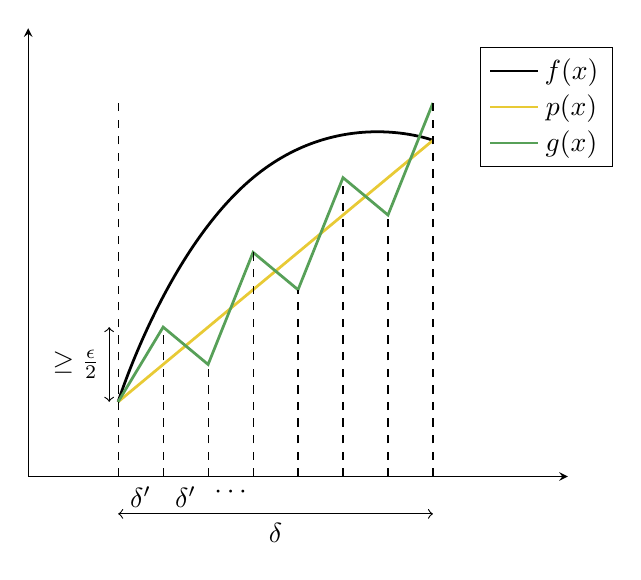
\begin{tikzpicture}
    \begin{axis}[
      axis y line = left,
      axis x line = bottom,
      ticks = none,
      clip = false,
      xmin = 0,
      xmax = 6,
      ymin = 0,
      ymax = 6,
      legend style={at={(axis cs:6.5,5.75)},anchor=north east},
      every axis plot/.append style={line width=1pt}
    ]
      \addplot [smooth, tension=1] 
        coordinates { 
          (1,1)
          (2.5,4)
          (4.5,4.5)
        }
      ;
      \addlegendentry{$f(x)$}

      \addplot[
        mark=none,
        color={rgb,255:red,232;green,202;blue,53}
      ] coordinates {
        (1, 1)
        (4.5, 4.5)
      };
      \addlegendentry{$p(x)$}

      \addplot[
        mark=none,
        color={rgb,255:red,87;green,160;blue,88}
      ] coordinates {
        (1, 1)
        (1.5, 2)
        (2, 1.5)
        (2.5, 3)
        (3, 2.5)
        (3.5, 4)
        (4, 3.5)
        (4.5, 5)
      };
      \addlegendentry{$g(x)$}

      \draw[dashed]
        (axis cs:1, 0) -- (axis cs:1, 5)
        (axis cs:1.5, 0) -- (axis cs:1.5, 2)
        (axis cs:2, 0) -- (axis cs:2, 1.5)
        (axis cs:2.5, 0) -- (axis cs:2.5, 3)
        (axis cs:3, 0) -- (axis cs:3, 2.5)
        (axis cs:3.5, 0) -- (axis cs:3.5, 4)
        (axis cs:4, 0) -- (axis cs:4, 3.5)
        (axis cs:4.5, 0) -- (axis cs:4.5, 5)
      ;

      \draw[<->]
        (axis cs: 1, -0.5) -- (axis cs:4.5, -0.5)
        node[midway, below] {$\delta$}
      ;

      \draw 
        (axis cs: 1.25, 0) node[below] {$\delta'$} 
        (axis cs: 1.75, 0) node[below] {$\delta'$} 
        (axis cs: 2.25, 0) node[below] {$\cdots$} 
      ;

      \draw[<->]
        (axis cs: 0.9, 1) -- (axis cs:0.9, 2)
        node[midway, left] {$\geq \frac{\epsilon}{2}$}
      ;
    \end{axis}
  \end{tikzpicture}
  \caption{
    Demonstrating adding zigzags to $p(x)$ to make its slope always big,
    but also maintaining continuity.
  }
  \label{chap8:fig:zigzags_px}
\end{figure}

We can choose $\delta' < \frac{n\epsilon}{2}$,
so then we have 
\begin{equation}
  \abs{g'(x)} \geq \abs{
    \frac{
      \epsilon/2
    }{
      \delta'
    }
  } > \frac{
    \epsilon/2
  }{
    n\epsilon/2
  } = n
\end{equation}
}
We have shown that the set of differentiable functions is 
the union of all $A_{m, n}$, which are nowhere-dense, and therefore 
it is a set of the first category.
}